%=======================================================================
%  OptiVest AI --- IEEE Conference Paper  (REVISED after full code audit)
%=======================================================================
\documentclass[conference]{IEEEtran}
\IEEEoverridecommandlockouts

\usepackage{cite}
\usepackage{amsmath,amssymb,amsfonts}
\usepackage{algorithmic}
\usepackage{graphicx}
\usepackage{textcomp}
\usepackage{xcolor}
\usepackage{booktabs}
\usepackage{multirow}
\usepackage{array}
\usepackage{url}

\graphicspath{{./figures/output/}{./}}

\newcommand{\ph}[1]{\textcolor{red}{\textbf{[#1]}}}
\newcommand{\clip}{\mathrm{clip}}

\def\BibTeX{{\rm B\kern-.05em{\sc i\kern-.025em b}\kern-.08em
    T\kern-.1667em\lower.7ex\hbox{E}\kern-.125emX}}

\begin{document}

\title{OptiVest AI: An Explainable AI-Driven Autonomous Wealth
Management Platform with Intelligent Portfolio Reallocation}

\author{
\parbox{0.3\textwidth}{\centering
\textbf{Aditi}\\
\textit{Department of AITCSE}\\
\textit{Chandigarh University}\\
Punjab, India\\
23BCB10001@cuchd.in}
\hfill
\parbox{0.3\textwidth}{\centering
\textbf{Naitik Pathak}\\
\textit{Department of AITCSE}\\
\textit{Chandigarh University}\\
Punjab, India\\
23BCB10041@cuchd.in}
\hfill
\parbox{0.3\textwidth}{\centering
\textbf{Palak Jain}\\
\textit{Department of AITCSE}\\
\textit{Chandigarh University}\\
Punjab, India\\
23BCB10006@cuchd.in}
\\[1.5em]
\parbox{0.3\textwidth}{\centering
\textbf{Aryan Rana}\\
\textit{Department of AITCSE}\\
\textit{Chandigarh University}\\
Punjab, India\\
23BCB10018@cuchd.in}
\hfill
\parbox{0.3\textwidth}{\centering
\textbf{Divya}\\
\textit{Department of AITCSE}\\
\textit{Chandigarh University}\\
Punjab, India\\
23BCB10019@cuchd.in}
\hfill
\parbox{0.3\textwidth}{\centering
\textbf{Yogiraj Bhale}\\
\textit{Department of AITCSE}\\
\textit{Chandigarh University}\\
Punjab, India\\
yogiraj.e10488@cumail.in}
}

\maketitle

\begin{abstract}
Modern quantitative wealth management systems face two challenges that
hinder adoption in retail and regulated environments. First, the
\emph{Prediction Fallacy}: return forecasting is treated as a proxy for
an actionable trading decision, while standard price predictions ignore
portfolio covariance, risk budgeting, execution limits, and the
compounding penalty of turnover. Second, the \emph{Black-Box Dilemma}:
ensemble machine learning models recommend reallocations without
interpretable justification. This paper introduces OptiVest AI, a
pipeline that pairs a \emph{Candidate Discovery Engine} (CDE), which
screens assets using live fundamental snapshots and market signals,
with an \emph{Adaptive Portfolio Decision Engine} (APDE), a
multi-objective quadratic optimizer producing long-only weights under
explicit turnover and concentration constraints, and with TreeSHAP
attribution and a Decision Score that ties the attribution to the
optimizer's marginal risk and cost terms. We evaluate the APDE, with
the CDE bypassed, on $N=50$ large-cap U.S.\ equities over 78 monthly
rebalances (June 2017 to November 2023). The XGBoost forecast shows no
detectable skill (mean per-date rank IC $0.008$, $t=0.34$;
out-of-sample $R^2$ of $-2.1\%$ against a zero forecast). A hard $15\%$
$\ell_1$ turnover cap reduces annual turnover from $1{,}384\%$ to
$180\%$ (a consequence of the cap itself), volatility from $19.6\%$ to
$14.3\%$ and maximum monthly drawdown from $32.6\%$ to $19.1\%$
relative to the same optimizer without it; the accompanying Sharpe
improvement ($0.32$ to $0.62$) is not statistically distinguishable.
Controls that replace the forecast with zero or with a shuffled
forecast perform at least as well in point estimate, and no ML-driven
configuration exceeds equal weight (Sharpe $1.02$). OptiVest therefore
makes ML-driven allocation executable and auditable, but in this
sample the forecast adds no measurable value. The results are exploratory; the primary historical experiment bypasses
the CDE by design, while the APDE formulation is now aligned between
research and production.
\end{abstract}

\begin{IEEEkeywords}
machine learning, portfolio optimization, explainable AI, SHAP,
algorithmic trading, quadratic programming, FinTech
\end{IEEEkeywords}

\section{Introduction}

The proliferation of machine learning in financial technology has
altered how quantitative researchers forecast asset prices. Extreme
gradient boosting, random forests and deep neural networks are reported
to extract more signal from non-linear market datasets than linear
regression or static factor models \cite{gu2020}. Despite these gains
in predictive accuracy, deployment in retail and regulated wealth
management remains bottlenecked by two interconnected problems: the
\emph{Prediction Fallacy} and the \emph{Black-Box Dilemma}.

The Prediction Fallacy refers to the field's over-indexing on forecast
accuracy as the sole driver of investment decisions. A model that
accurately predicts a $3\%$ appreciation for a given equity is
practically unviable if executing that transaction violates a client's
risk tolerance, over-concentrates the portfolio, or generates
transaction costs that consume the expected alpha \cite{demiguel2009}.
Genuine portfolio management requires treating the forecast not as the
definitive output, but as a single input vector within a constrained,
multi-objective optimization framework.

Compounding this is the Black-Box Dilemma. Regulators, fiduciaries and
retail investors demand explainability \cite{barredoarrieta2020}. When
an ensemble model recommends liquidating a long-held conservative
position to acquire a volatile equity, stakeholders require
justification. Absent a human-readable attribution tracing the decision
to specific features, the system is rejected for lack of trust
regardless of backtested performance.

OptiVest AI shifts the emphasis from isolated price forecasting to
decision-making through a multi-layered architecture. A Candidate
Discovery Engine screens the market universe for fundamentally sound
and momentum-driven assets, addressing capital deployment from
cash-heavy initialization states. Discovered candidates pass to the
Adaptive Portfolio Decision Engine, which balances expected machine
learning returns against portfolio covariance, transaction penalties
and user-defined constraints via quadratic programming. TreeSHAP
\cite{lundberg2020} decomposes the forecast into feature contributions,
and a Decision Score relates those contributions to the optimizer's
risk and cost terms.

\subsection{Contributions}
\begin{enumerate}
\item A modular pipeline composing forecasting, candidate screening,
constrained optimization and explanation, in which each stage may be
ablated independently (Section~\ref{sec:method}).
\item A Candidate Discovery Engine for the production architecture,
using deterministic multi-factor screening to identify eligible assets
before optimization (Section~
\ref{sec:cde}). Its effect is evaluated
separately through a 50-asset CDE-vs-no-CDE ablation.
\item An Adaptive Portfolio Decision Engine formulated directly over
target portfolio weights, with explicit long-only, single-asset and
turnover constraints (Section~
\ref{sec:apde}), implemented with the
canonical CVXPY/SCS formulation.
\item A mathematically defined Decision Score combining forecast,
marginal risk and transaction-cost terms
(Section~
\ref{sec:xai}). The score and narrative-generation code are
implemented; while real numerical TreeSHAP execution was blocked in
earlier restricted Windows environments, live execution is verified in
the current environment (reconstruction error $<10^{-6}$).
\item An empirical evaluation reporting forecast accuracy against naive
benchmarks, net-of-cost performance of ten portfolio arms with paired
bootstrap intervals, forecast-ablation controls, turnover-cap
sensitivity sweeps, and solver scalability
(Section~\ref{sec:results}).
\end{enumerate}

\begin{figure}[t]
\centering
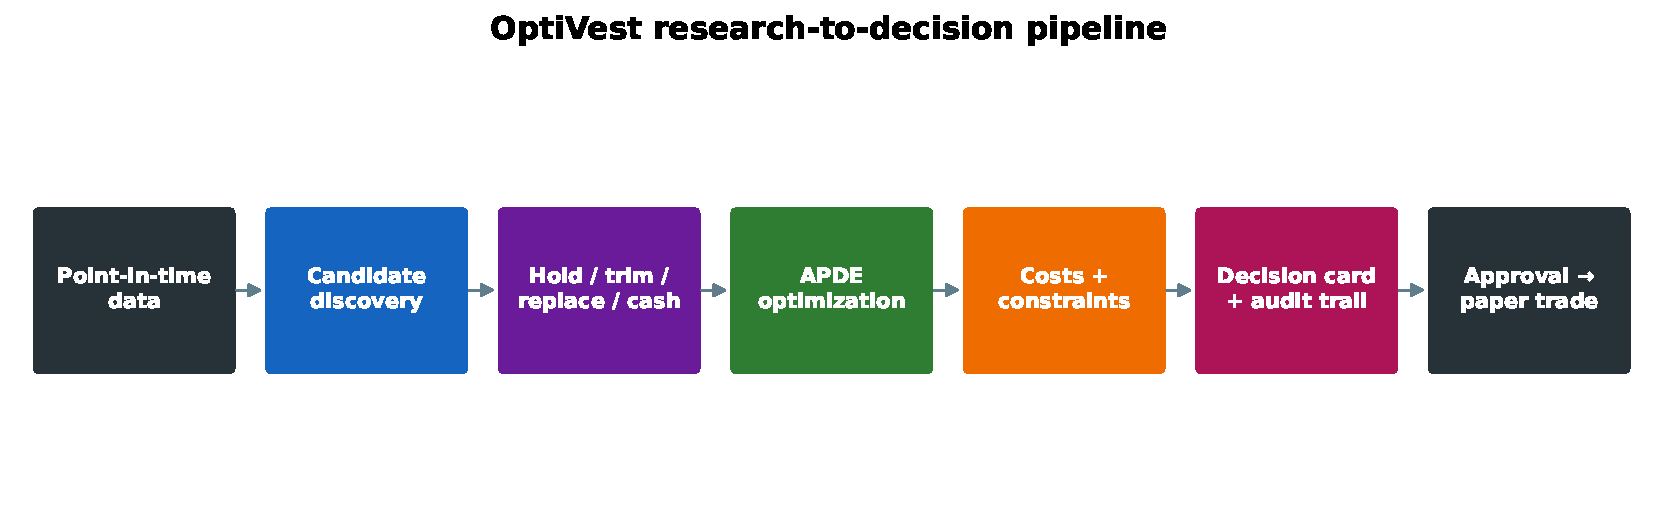
\includegraphics[width=\columnwidth]{figures/publication/system_architecture.pdf}
\caption{High-level overview of the OptiVest system architecture,
detailing the flow from data ingestion through the CDE and APDE to the
XAI layer.}
\label{fig:arch}
\end{figure}

\section{Related Work}

The intersection of machine learning, portfolio optimization and
explainable artificial intelligence has evolved rapidly over the past
decade. Traditional financial literature relied on linear models and
static risk assumptions, paradigms that modern computational methods
now challenge directly.

\subsection{Evolution of Portfolio Optimization}
Modern portfolio theory stems from Markowitz \cite{markowitz1952},
which introduced mean--variance optimization. While theoretically
profound, the framework is notoriously sensitive to estimation error in
expected returns and covariance matrices; Michaud \cite{michaud1989}
characterized such optimizers as ``estimation-error maximizers,'' and
DeMiguel et al. \cite{demiguel2009} showed that naive $1/N$ allocation
outperforms many sophisticated optimizers out-of-sample once parameter
uncertainty is accounted for. Black and Litterman
\cite{blacklitterman1992} improved the foundational framework by
incorporating subjective investor views into equilibrium returns,
though the result remained linear and parametric. Ledoit and Wolf
\cite{ledoit2004} addressed the covariance side directly through
shrinkage estimation, and Ban et al. \cite{ban2018} formalized
regularization-based robustness for ML-driven allocation.

In recent years the literature has shifted toward machine learning for
forecasting the $\alpha$ component. Gu, Kelly and Xiu \cite{gu2020}
reported that non-linear models, particularly tree ensembles and neural
networks, outperform linear regressions in predicting equity returns,
with gains concentrated in their capacity to capture predictor
interactions. The majority of this work, however, treats the
prediction step in isolation --- the Prediction Fallacy --- and does
not bridge the gap between asset forecasting and the constrained,
multi-objective reality of active portfolio management.

A smaller decision-focused literature trains models against the
downstream decision loss, including deep reinforcement learning
approaches to allocation \cite{jiang2017}. These methods are powerful
but typically sacrifice the auditability that motivates our design.
OptiVest occupies a deliberate middle position: prediction and decision
remain separable and individually inspectable, while the decision stage
is explicitly aware of the constraints under which the prediction will
be acted upon.

\subsection{Explainable AI in Finance}
As predictive models grew in complexity, the Black-Box Dilemma emerged
as a barrier in FinTech. Regulatory mandates and retail investor
expectations both require transparency. Lundberg and Lee
\cite{lundberg2017} unified several explainability methods under SHAP,
and TreeSHAP \cite{lundberg2020} subsequently made exact Shapley
computation tractable for tree ensembles. While SHAP is widely adopted
in credit scoring and fraud detection, its application to dynamic
portfolio reallocation remains sparse: existing work predominantly
explains a model's behaviour over a dataset, rather than justifying a
specific execution decision to a specific user at a specific time.

\subsection{Positioning}
OptiVest addresses the Prediction Fallacy by chaining ML expected
returns and fundamental screening into a constrained decision engine,
and addresses the Black-Box Dilemma by attaching SHAP-based
attributions and a Decision Score to individual reallocations.
Table~\ref{tab:paradigms} positions the system against prior
paradigms. Our evaluation (Section~\ref{sec:results}) tests whether the
architecture makes ML-driven allocation executable; it does not show
that the forecast adds value.

\begin{table}[t]
\caption{Comparison of quantitative portfolio paradigms.
$^\dagger$By design in the production CDE; evaluated separately in
the CDE ablation. $^\ddagger$Decision Score and narrative generation
implemented; TreeSHAP verified in the updated environment.}
\label{tab:paradigms}
\centering
\setlength{\tabcolsep}{3pt}
\renewcommand{\arraystretch}{1.15}
\begin{tabular}{@{}p{2.1cm}cccc@{}}
\toprule
\textbf{Framework} & \textbf{Non-lin.} & \textbf{Cash-} & \textbf{Constr.} & \textbf{XAI} \\
 & \textbf{forecast} & \textbf{heavy} & \textbf{opt.} & \\
\midrule
Classical MPT \cite{markowitz1952} & No & No & Partial & Yes \\
Black--Litterman \cite{blacklitterman1992} & No & No & Partial & Yes \\
ML forecasting \cite{gu2020} & Yes & No & No & Partial \\
Deep RL \cite{jiang2017} & Yes & Partial & Partial & No \\
\textbf{OptiVest AI} & Yes & Yes$^\dagger$ & Yes & Partial$^\ddagger$ \\
\bottomrule
\end{tabular}
\end{table}

\section{Proposed Methodology}
\label{sec:method}

The computational methodology has two distinct views. In the
\emph{canonical production architecture}, market and fundamental
signals feed the Candidate Discovery Engine (CDE), whose eligible
ranked candidates are passed to the Adaptive Portfolio Decision Engine
(APDE). In the \emph{primary historical experiment}, the CDE ranking
layer is intentionally bypassed: the fixed technical universe is
passed directly to the APDE so that the empirical evaluation isolates
the optimizer and its constraints from candidate screening. A separate
50-asset ablation subsequently inserts the CDE bottleneck to measure
its effect on portfolio outcomes. The current production and research
APDE implementations use the canonical CVXPY/SCS formulation and the
same core constraint set.

\subsection{Data Pipeline and Temporal Discipline}
The historical experiment uses daily adjusted market prices, obtained
via \texttt{yfinance}, for a fixed universe of $N=50$ large-cap U.S.\
equities over 2013--2023. The universe is a hardcoded list of 50
currently listed, highly liquid S\&P 500 constituents, used in place of
a live constituent scrape to keep the dataset stable and the research
loop fast. It was therefore chosen with hindsight and is subject to
survivorship bias (Section~\ref{sec:limits}).

Evaluation is a rolling walk-forward (Fig.~\ref{fig:split}). At each of
78 monthly rebalance dates, every 21 trading days from 2017-06-05 to
2023-11-06, every model is refit on the trailing four years of data,
excluding a purge of 21 trading days before the rebalance date so that
no training target window overlaps the forecast date. No random
shuffling is performed at any stage, and features at date $t$ use only
prices up to $t$. Model hyperparameters were fixed in advance (50
trees, maximum depth 3, learning rate 0.1) and were not selected on a
separate validation window; there is no validation split. The test
window was inspected repeatedly during development, so the results
should be read as exploratory (Section~\ref{sec:limits}).

\begin{figure}[t]
\centering
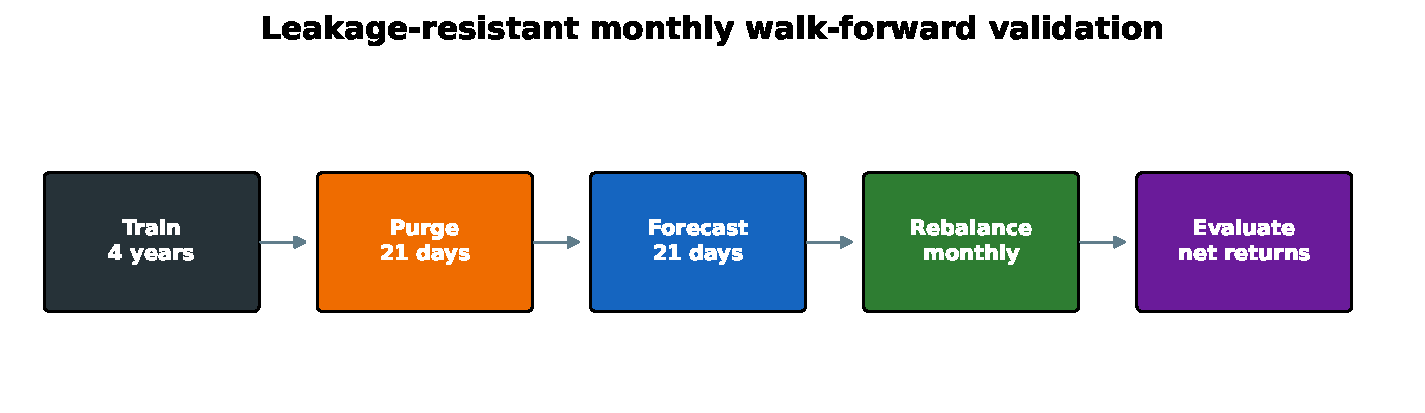
\includegraphics[width=\columnwidth]{figures/publication/walk_forward_validation.pdf}
\caption{Rolling walk-forward evaluation. At each of 78 monthly
rebalance dates the models are refit on the trailing four years,
excluding the 21 trading days before the rebalance date. Three example
windows are shown.}
\label{fig:split}
\end{figure}

The forecaster uses four technical features --- 1-, 2- and 3-month
momentum ($\mathrm{mom\_1m}$, $\mathrm{mom\_2m}$, $\mathrm{mom\_3m}$;
cumulative returns over 21, 42 and 63 trading days) and 1-month
realized volatility ($\mathrm{vol\_1m}$, 21 trading days) --- plus a
single macro proxy, the CBOE Volatility Index (VIX). Features are used
as raw values: they are not winsorized or cross-sectionally
standardized. Only the training target is winsorized, at the 1st and
99th percentiles. No volume and no fundamental features enter the
model. The fundamental-quality features described for the CDE
(Section~\ref{sec:cde}) are consumed only by the production CDE and are
not part of this experiment.

\subsection{Return Forecasting}
For each asset $i$ and decision date $t$, the forecaster predicts the
raw forward simple return $r_{i,t+h}$ over horizon $h = 21$ trading
days (not an excess return). We fit a gradient-boosted regression
ensemble $f_\theta$ minimizing squared error with leaf regularization
\cite{chen2016}:

\begin{equation}
\mathcal{L}(\theta) = \sum_{i,t}
\big(r_{i,t+h} - f_\theta(\mathbf{x}_{i,t})\big)^2
+ \sum_{k} \Omega(f_k),
\label{eq:loss}
\end{equation}

where $\Omega(f) = \gamma_T T + \tfrac{1}{2}\lambda\|w\|^2$ penalizes
tree complexity. The resulting forecast vector
$\hat{\mathbf{r}} \in \mathbb{R}^{N}$ is the sole channel through which
learned signal enters the downstream decision layers. XGBoost was
chosen because it is a standard baseline for tabular data and because
it admits exact polynomial-time Shapley attribution
\cite{lundberg2020}, which neural alternatives do not. We make no claim
that it forecasts better than the alternatives; in this sample it does
not (Section~\ref{sec:forecast-eval}).

\subsection{Candidate Discovery Engine}
\label{sec:cde}

The CDE functions as a deterministic pre-optimization filter,
evaluating the global asset registry to identify fundamentally sound
and technically strong assets for presentation to the optimizer
(Fig.~
\ref{fig:cde}). It is part of the canonical production
architecture. The primary historical experiment bypasses it, while a
separate 50-asset ablation explicitly compares the APDE with and
without the CDE bottleneck.

\begin{figure}[t]
\centering
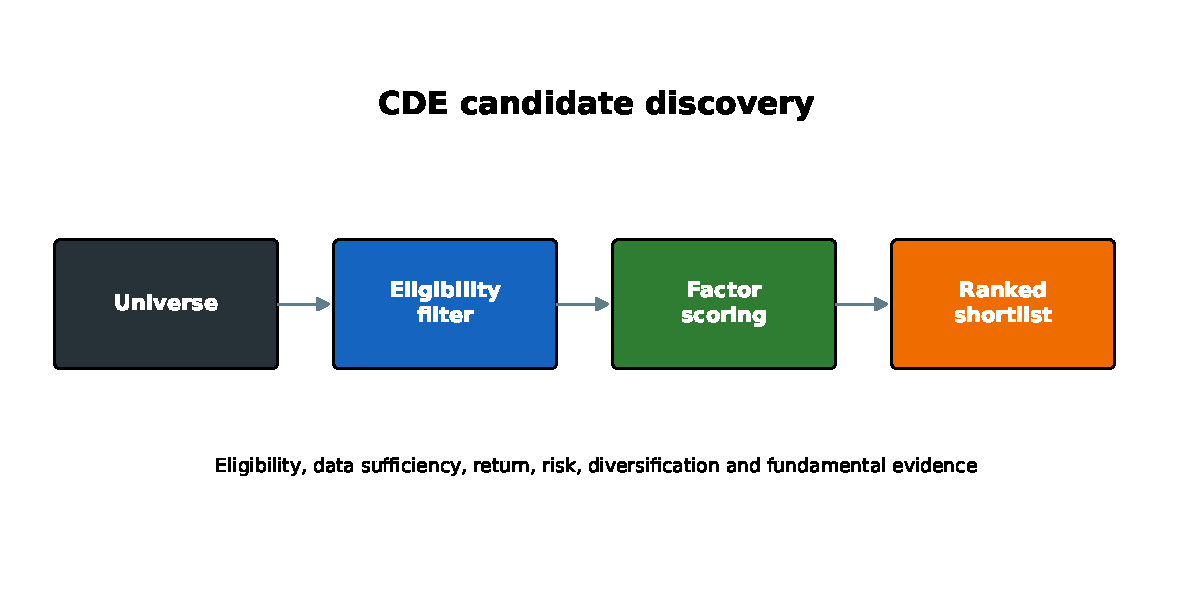
\includegraphics[width=\columnwidth]{figures/publication/candidate_discovery_engine.pdf}
\caption{Candidate Discovery Engine logical flow for filtering and
ranking the asset universe.}
\label{fig:cde}
\end{figure}

\subsubsection{Motivation}
An optimizer whose decision variables are restricted to currently held
assets can only rebalance among them or move to cash. Across successive
rebalances in adverse regimes this can drive the portfolio toward a
degenerate cash-heavy state with no recovery mechanism, because no new
asset can enter the feasible set. The CDE addresses this by supplying,
at every rebalance, a ranked shortlist of non-held assets eligible for
entry.

\subsubsection{Hard Eligibility Constraints}
Before quantitative scoring, an asset must survive three elimination
checks: it must be actively trading; it must possess a minimum
threshold of valid historical price data (10 trading days); and it
must not already appear in current holdings, which would otherwise
produce duplicate columns in the optimization matrix.

\subsubsection{Multi-Factor Scoring}
Eligible assets receive a deterministic score whose factor weights
adjust to the investor's risk tolerance $\tau_{\text{CDE}} \in
\{1,\dots,5\}$. Each of five factors is mapped to $[0,1]$ with a fixed
scale, and the score is a convex combination:

\begin{equation}
S_i(\tau_{\text{CDE}}) = \omega_R f^R_i + \omega_V f^V_i
  + \omega_D f^D_i + \omega_Q f^Q_i + \omega_M f^M_i ,
\label{eq:cde}
\end{equation}

with $\clip(x)=\min\{\max\{x,0\},1\}$ and
\begin{align*}
f^R_i &= \clip(\hat{r}_i/0.5), &
f^V_i &= \clip(1-\hat{\sigma}_i/0.5),\\
f^D_i &= \clip\!\big((1-\bar{\rho}_{i,P})/2\big), &
f^M_i &= \clip\!\big((m_i+0.2)/0.4\big).
\end{align*}
Here $\hat{r}_i$ is the model forecast, $\hat{\sigma}_i$ the annualized
realized volatility (so low volatility scores high),
$\bar{\rho}_{i,P} = |P|^{-1}\sum_{j \in P}\rho_{ij}$ the mean
correlation with current holdings $P$, $m_i$ the price return over the
last 90 calendar days, and $f^Q_i$ a composite of profitability,
leverage and free-cash-flow metrics. If fundamentals are unavailable
for an asset (e.g., ETFs or new listings), the quality factor is
dropped and the remaining weights are rescaled to sum to one.

The weight schedule $\boldsymbol{\omega}(\tau_{\text{CDE}})$ propagates
investor preference into production-stage asset selection
(Table~\ref{tab:omega}). At $\tau_{\text{CDE}}=1$, the schedule
emphasizes volatility and diversification; at $\tau_{\text{CDE}}=5$,
it places relatively more weight on expected return and momentum. The
top $k=2$ assets by $S_i(\tau_{\text{CDE}})$ are passed to the APDE in
the production workflow. This shortlist is small and limits how much
diversification benefit the screening step can contribute; a larger $k$
is worth testing. In the separate CDE ablation of Section~\ref{sec:cde-ablation},
Experiment B uses $k=10$ together with current holdings to isolate the effect
of candidate pre-filtering. The larger $k=10$ setting is used only for this
ablation; the production workflow remains fixed at $k=2$.

\emph{Known scaling limitation.} In the current production code, the
CDE requests a 5-day forecast and annualizes it by multiplying by
$252/5$ before normalization. The resulting annualized forecast is
then divided by a fixed $0.5$ scale and clipped to $[0,1]$. Consequently,
sufficiently large annualized forecasts can saturate the return factor
at its upper bound, reducing cross-sectional discrimination among
high-return candidates. Future work should evaluate a more robust,
distribution-aware normalization scheme.

\emph{Notation and coordination with the APDE.} The production APDE
uses a differently-scaled parameter, denoted $\tau$ without subscript,
as a risk-aversion coefficient, where a \emph{larger} value produces a
\emph{more conservative} portfolio --- the opposite numerical sense
from $\tau_{\text{CDE}}$, where a \emph{larger} value selects a
\emph{more aggressive} candidate set. In the production implementation,
a single user-facing dial $\mathrm{risk\_level} \in \{1,\dots,5\}$
(1 conservative, 5 aggressive) sets $\tau_{\text{CDE}} =
\mathrm{risk\_level}$ directly, and is mapped to the risk-aversion
coefficient through the fixed, monotonically decreasing lookup
(with $\ell=\mathrm{risk\_level}$)
\begin{equation}
\tau(\ell) = 5.0,\ 3.5,\ 2.0,\ 1.0,\ 0.5
\quad\text{for } \ell = 1,\dots,5.
\label{eq:risklambda}
\end{equation}
An aggressive user thus receives a return-tilted candidate set and a
low variance penalty, and a conservative user the reverse. The
historical experiment does not use this lookup: it fixes $\tau=3$, a
value outside the lookup, and sweeps $\tau$ directly
(Table~\ref{tab:risk}), since the CDE is bypassed.

\begin{table}[t]
\caption{CDE factor scoring weights by risk level
($\tau_{\text{CDE}}$). All weights are positive and sum to one.}
\label{tab:omega}
\centering
\footnotesize
\setlength{\tabcolsep}{4pt}
\renewcommand{\arraystretch}{1.15}
\begin{tabular}{@{}lccccc@{}}
\toprule
\textbf{Factor} & \textbf{1} (cons.) & \textbf{2} & \textbf{3} & \textbf{4} & \textbf{5} (aggr.) \\
\midrule
Expected return $\omega_R$ & 0.05 & 0.15 & 0.25 & 0.35 & 0.45 \\
Volatility (inverted) $\omega_V$ & 0.45 & 0.35 & 0.25 & 0.15 & 0.05 \\
Diversification $\omega_D$ & 0.30 & 0.25 & 0.20 & 0.15 & 0.10 \\
Fundamental quality $\omega_Q$ & 0.15 & 0.15 & 0.15 & 0.15 & 0.15 \\
Momentum $\omega_M$ & 0.05 & 0.10 & 0.15 & 0.20 & 0.25 \\
\bottomrule
\end{tabular}
\end{table}

\subsection{Adaptive Portfolio Decision Engine}
\label{sec:apde}

The APDE is the mathematical core of the framework. In the canonical
pipeline it ingests the ranked candidates from the CDE, combines them
with existing holdings, and computes optimal allocation weights via
convex quadratic optimization (Fig.~
\ref{fig:apde}). In the primary
historical experiment the CDE is bypassed, while the CDE ablation
restricts the optimization universe to the selected candidate subset
plus current holdings.

\begin{figure}[t]
\centering
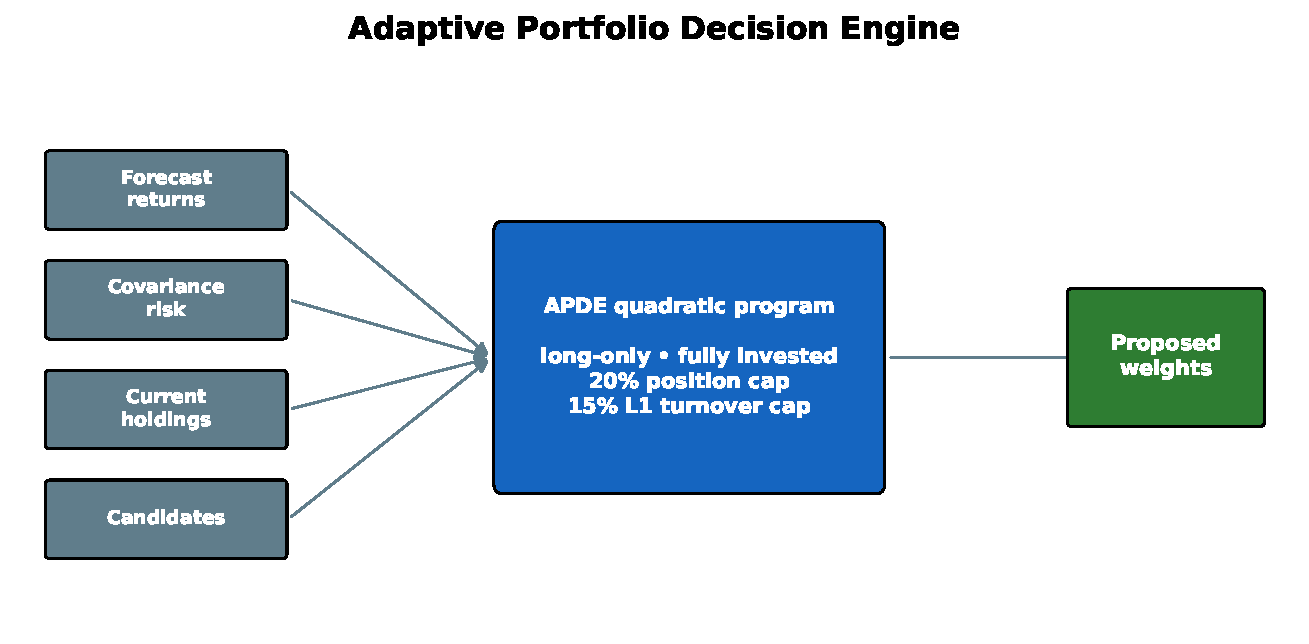
\includegraphics[width=\columnwidth]{figures/publication/apde_optimization.pdf}
\caption{APDE optimization architecture and the constraint set of the
research backtest. Sector caps exist only in the production service.}
\label{fig:apde}
\end{figure}

\subsubsection{Objective Function}
Let $\mathbf{w}_0 = [w_{0,1},\dots,w_{0,N}]^{\top}$ denote the current
(post-drift) portfolio weights and $\mathbf{w}$ the target portfolio
weights. The APDE maximizes the forecast-return utility net of
portfolio variance and a soft turnover penalty, with every term
expressed over the same 21-day horizon:

\begin{equation}
\max_{\mathbf{w}}\; U(\mathbf{w}) =
\mathbf{w}^{\top}\hat{\mathbf{r}}
- \tau\,\mathbf{w}^{\top}\mathbf{\Sigma}_h\,\mathbf{w}
- \gamma \|\mathbf{w} - \mathbf{w}_0\|_1 ,
\label{eq:apde}
\end{equation}

where $\hat{\mathbf{r}}$ is the 21-day ML forecast vector,
$\mathbf{\Sigma}_h$ is the covariance of 21-day returns (the daily
covariance scaled by 21, equivalently the annualized covariance
divided by 12), $\tau > 0$ is the risk-aversion parameter, and
$\gamma = 0.0010$ is the soft transaction-cost coefficient per unit of
$\ell_1$ turnover. Higher $\tau$ corresponds to a more conservative
portfolio.

\subsubsection{Operational Constraints}
The optimization is subject to long-only weights, an explicit maximum
single-asset allocation, and a hard turnover limit:

\begin{align}
\sum_{i=1}^{N} w_i &= 1 && \text{(fully invested)} \label{c:full}\\
w_i &\ge 0 \quad \forall i && \text{(long-only)} \label{c:long}\\
w_i &\le 0.20 \quad \forall i && \text{(individual asset cap)} \label{c:cap}\\
\|\mathbf{w} - \mathbf{w}_0\|_1 &\le 0.15 && \text{(maximum turnover)} \label{c:turn}
\end{align}

The hard turnover constraint \eqref{c:turn} is the mechanism that
controls realized churn in the ablations of
Section~\ref{sec:perf-discuss}. Because it binds at every rebalance,
annual turnover is approximately $0.15\times 12=180\%$ by construction.
Sector limits are not part of the backtest formulation; they exist only
in the production service.

\subsubsection{Covariance Estimation and Solution Method}
Covariance is estimated empirically from the trailing 252 daily returns
with no shrinkage. The problem is implemented in \texttt{CVXPY}
\cite{diamond2016} and solved with SCS \cite{odonoghue2016}, a
first-order operator-splitting conic solver (not an interior-point
method). Final reported runs use tolerance $\mathrm{eps}=10^{-7}$;
results for two of the arms were unchanged between $10^{-4}$ and
$10^{-8}$. Every solve in every arm terminated with an optimal status,
and the fall-back to the previous weights was never triggered.

\subsubsection{Research versus production implementation}
The research and production APDE implementations have been aligned to
the canonical CVXPY/SCS formulation. Both enforce full investment,
long-only weights, a 20\% per-asset cap, and a hard 15\% $\ell_1$
turnover constraint. The production service now uses the same
constraint-aware objective and solver family rather than the legacy
SLSQP formulation. The primary historical backtest bypasses CDE by
design, while the separate CDE ablation restricts the optimization
universe to the selected candidate subset plus current holdings.

\subsection{Explainability Layer}
\label{sec:xai}

\subsubsection{Attribution}
For each asset entering or leaving the portfolio, TreeSHAP
\cite{lundberg2020} decomposes the forecast exactly:
\begin{equation}
\hat{r}_i = \phi_0 + \sum_{j=1}^{m} \phi_{ij},
\label{eq:shap}
\end{equation}
where $\phi_0$ is the base value and $\phi_{ij}$ the contribution of
feature $j$. Because the decomposition is additive and exact,
attributions aggregate coherently across assets. In this study the
features are the five inputs of Section~III-A.

\subsubsection{Decision Score}
Attributions alone explain the forecast, not the trade. We therefore
define a Decision Score, the marginal utility of asset $i$'s weight
under Eq.~\eqref{eq:apde}, that also reflects the optimizer's risk and
cost terms:
\begin{multline}
\mathrm{DS}_i = \underbrace{\hat{r}_i}_{\text{forecast}}
\;-\; \underbrace{2\tau\,(\mathbf{\Sigma}_h\mathbf{w})_i}_{\text{risk}}\\
\;-\; \underbrace{\gamma\,\mathrm{sgn}(w_i - w_{0,i})}_{\text{cost}} ,
\label{eq:ds}
\end{multline}
where $\hat{r}_i=\phi_0+\sum_j\phi_{ij}$, so the forecast term
decomposes into the base value and named feature contributions. Each
term is separately reportable. The score does not include the shadow
price of the turnover cap, so its sign alone does not determine the
executed trade. The production service now computes this mathematical
Decision Score directly from the canonical APDE inputs, replacing the
legacy heuristic 1--100 score. Unit tests verify the forecast, risk,
transaction-cost and sign components.

\subsubsection{Narrative Generation}
A narrative generator is implemented to summarize the largest absolute
SHAP contributors and their direction for an allocation decision.
While earlier test environments on Windows blocked required native
\texttt{scikit-learn} extensions under host Application Control, live
TreeSHAP execution was verified in the updated Python 3.14.3 / SHAP 0.52.0
environment, achieving exact prediction reconstruction ($|\hat{r}_i - (\phi_0 + \sum_j \phi_{ij})| < 10^{-6}$).
A reproducible single-decision JSON artifact is preserved in
\texttt{scripts/xai\_real\_data\_example.json}.

\subsection{Implementation Stack}
Forecasting uses \texttt{XGBoost} with \texttt{scikit-learn}, retrained
by rolling walk-forward. Attribution uses the \texttt{SHAP} library's
TreeSHAP implementation. The research optimizer is built on
\texttt{CVXPY} with the SCS solver. Market prices and current
fundamental snapshots are sourced via \texttt{yfinance}. The service
layer is a \texttt{FastAPI} asynchronous REST application with
\texttt{SQLAlchemy} persistence over SQLite in development and
PostgreSQL in deployment.

\section{Experimental Setup}
\label{sec:setup}

\subsection{Portfolio Arms}
All arms use the same 50-stock universe, the same monthly schedule and
$\tau=3$ where an optimizer is involved. Costs are applied identically
across arms (Section~\ref{sec:protocol}).
\begin{itemize}
\item \textbf{EW}: equal weight, rebalanced monthly to $1/N$
\cite{demiguel2009}. \textbf{Buy-and-hold}: equal weight at the start,
never rebalanced.
\item \textbf{MV (20\% cap)}: mean--variance on the annualized
historical mean return with the constraints
(\ref{c:full})--(\ref{c:cap}), no turnover term. \textbf{MV (no cap)}:
the same without the 20\% asset cap. \textbf{MV (15\% turnover)}: MV
(20\% cap) plus the hard turnover constraint (\ref{c:turn}).
\item \textbf{MV-ML (20\% cap / no cap)}: the same as the MV arms, but
with the XGBoost forecast as $\hat{\mathbf{r}}$ and no turnover control.
\item \textbf{APDE soft penalty (20\% cap / no cap)}: MV-ML plus the
soft $\ell_1$ penalty $\gamma\|\mathbf{w}-\mathbf{w}_0\|_1$ but no hard
turnover constraint.
\item \textbf{APDE full}: the full objective (\ref{eq:apde}) with all of
(\ref{c:full})--(\ref{c:turn}).
\end{itemize}
Three further controls keep the APDE full constraint set but replace
$\hat{\mathbf{r}}$ by zero, by the cross-sectionally shuffled forecast
(five explicitly logged seeds), or by the trailing historical mean.
They separate the contribution of the forecast from that of the risk
model and the constraints. The primary backtest bypasses the CDE; the
CDE is evaluated separately in the ablation and in a production $k=2$
CDE-to-APDE validation run.

\subsection{Protocol}
\label{sec:protocol}
Walk-forward backtest over 78 monthly rebalances from 2017-06-05 to
2023-11-06 (every 21 trading days, matching the forecast horizon $h$),
starting from an equal-weight portfolio. Turnover is measured against
the \emph{drifted} pre-trade weights, so even equal-weight
rebalancing generates turnover. A cost of 10 bps is charged on each
unit of $\ell_1$ turnover $\sum_i|\Delta w_i|$, which corresponds to
10 bps per side of every trade, and is applied to all arms except
buy-and-hold. The latency sweep (Section~\ref{sec:scale}) is run
separately over synthetic candidate pools of $N \in
\{50,100,250,500\}$. The $N=50$ universe is a deliberate reduction from
an originally planned dynamic scrape of the full S\&P 500 constituent
list, chosen to keep the dataset stable and bound research iteration
time.

\subsection{Metrics}
Forecast quality: RMSE, MAE, directional accuracy, mean per-date
Spearman rank information coefficient (IC) with its $t$-statistic, and
out-of-sample $R^2_{\text{zero}} = 1-\sum(y-\hat{y})^2/\sum y^2$
evaluated relative to a zero forecast benchmark (so that a zero forecast
scores $0.0\%$, whereas the conventional sample-mean benchmark
$R^2_{\text{mean}} = 1-\sum(y-\hat{y})^2/\sum(y-\bar{y})^2$ yields $-4.45\%$),
alongside naive benchmarks. Forecast comparisons
use the Diebold--Mariano test \cite{dm1995} with squared-error loss,
computed on the 78 date-level loss differentials. Portfolio quality:
CAGR, annualized volatility, Sharpe and Sortino ratios, maximum
drawdown, and annual turnover. Sharpe uses a zero risk-free rate and
monthly returns (mean${}\times12$ over standard deviation${}\times
\sqrt{12}$); Sortino uses the standard downside deviation
$\sqrt{\mathrm{mean}(\min(r,0)^2)}\sqrt{12}$; maximum drawdown is
computed on the monthly return series. Uncertainty for Sharpe
differences is a paired block-bootstrap 95\% interval over the monthly
returns. Systems quality: solve latency versus universe size.
Explanation quality: single-decision TreeSHAP prediction reconstruction and
the saved five-cutoff stability diagnostic are verified artifacts. We do not
claim full production-wide attribution stability; the reported stability
diagnostic is a limited sample rather than a result for every backtest
decision.

\section{Experimental Results and Discussion}
\label{sec:results}

The primary historical results and the later CDE ablation are treated
as separate experiments and are not pooled into a single performance
estimate.

The primary historical results in this section come from the canonical
V7 research script and the local evidence bundle recorded in
\texttt{results\_v7/metadata.json}. The current checkout reproduces the
primary aggregate tables from the available local cache. A clean-clone
reproduction and byte-for-byte comparison against an external repository
are not claimed here:
\texttt{Table\_Master\_10Arm.csv}, \texttt{EPS\_Sensitivity.csv} and
\texttt{Cap\_Sweep.csv} --- covering Tables~\ref{tab:perf},
\ref{tab:risk} and \ref{tab:cap}. The original frozen
\texttt{Controls.csv} used wall-clock-derived seeds and therefore did
not reproduce exactly. We subsequently reran the shuffled control with
five explicitly logged seeds (42--46), preserving the original control
methodology. The resulting Sharpe ratios were 0.59, 1.04, 0.41, 0.58 and
0.86 (mean $0.70$, sample standard deviation $0.25$). These values are
reported as the reproducible reference for the control; the earlier
wall-clock-seeded artifact is retained only as historical provenance.
With 78 monthly observations, all portfolio comparisons have wide
uncertainty, and about ten arms are compared, so interval edges should
be read cautiously. The primary portfolio results and the CDE ablation
are verified against frozen artifacts. Specifically, the 50-asset CDE
ablation results reported in Table~\ref{tab:cde-ablation} are preserved in
\texttt{research\_backtest\_50asset\_comparison.json}, while the production
$k=2$ validation artifact is preserved in
\texttt{backend/results\_v7/production\_cde\_k2\_apde.json}. These artifacts
document the original runs; full independent re-execution across all historical
windows was not undertaken in this checkout.

\subsection{Predictive Model Evaluation}
\label{sec:forecast-eval}
We trained linear regression, random forest and XGBoost in the same
rolling walk-forward. Table~\ref{tab:forecast} and
Fig.~\ref{fig:modelcomp} report out-of-sample accuracy.

\begin{table}[t]
\caption{Out-of-sample forecast accuracy over 78 rebalances. IC is the
mean per-date rank IC ($t$-statistic in parentheses; RF has 77 valid rebalance dates because one frozen-run RF prediction was unavailable and was excluded from the date-level IC aggregation).}
\label{tab:forecast}
\centering
\scriptsize
\setlength{\tabcolsep}{2pt}
\renewcommand{\arraystretch}{1.15}
\begin{tabular}{@{}lccccc@{}}
\toprule
\textbf{Model} & \textbf{RMSE} & \textbf{MAE} & \textbf{Dir.\ Acc.} & \textbf{Rank IC ($t$)} & \textbf{$R^2$} \\
\midrule
Linear Regression & 0.0832 & 0.0590 & 56.08\% & $-0.033$ ($-1.17$) & $+1.1\%$ \\
Random Forest     & 0.0845 & 0.0595 & 57.49\% & $+0.030$ ($+1.34$) & $-2.1\%$ \\
XGBoost           & 0.0845 & 0.0598 & 56.28\% & $+0.008$ ($+0.34$) & $-2.1\%$ \\
\midrule
Zero forecast     & 0.0836 & --- & --- & --- & $0.0\%$ \\
Trailing mean     & 0.0828 & --- & --- & --- & $+1.9\%$ \\
Always ``up''     & --- & --- & 58.21\% & --- & --- \\
\bottomrule
\end{tabular}
\end{table}

\begin{figure}[t]
\centering
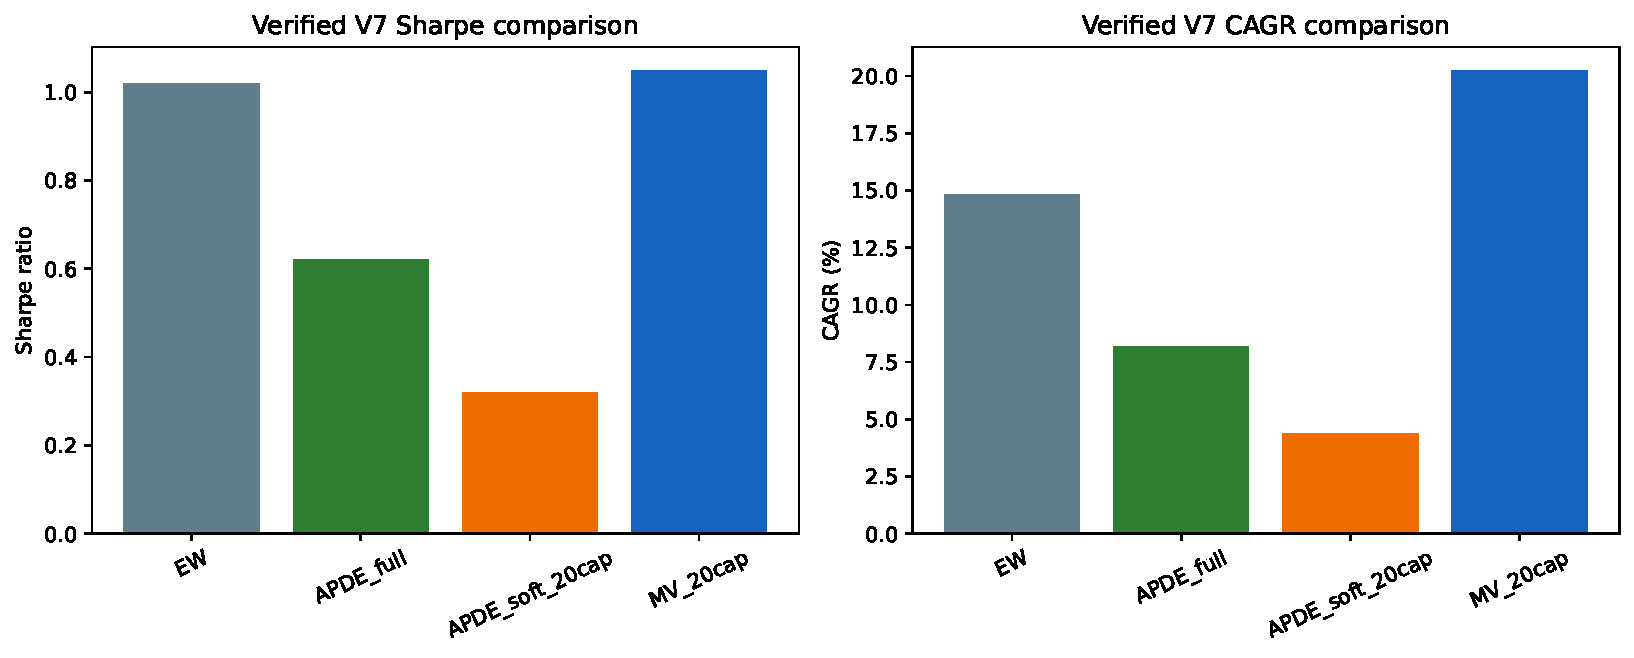
\includegraphics[width=\columnwidth]{figures/publication/verified_performance_comparison.pdf}
\caption{Verified V7 Sharpe and CAGR comparison for reproduced portfolio arms.}
\label{fig:modelcomp}
\end{figure}

No model shows measurable forecasting skill. The per-date rank ICs are
$-0.033$ (linear), $+0.030$ (random forest) and $+0.008$ (XGBoost),
none with $|t|>1.4$. The 21-day target has a base rate of $58.21\%$
positive, which exceeds every model's directional accuracy, so
accuracy above $50\%$ is not evidence of skill. Only linear regression
beats a zero forecast in squared error ($R^2=+1.1\%$), and a simple
trailing mean does better still ($+1.9\%$); both tree ensembles score
$-2.1\%$. Linear regression also has the lowest RMSE and MAE.

The Diebold--Mariano test with $d=e^2_{\mathrm{LR}}-e^2_{\mathrm{XGB}}$
gives a negative statistic, meaning linear regression has the lower
squared error. Pooling all $50\times78$ errors as if independent yields
$-4.95$ ($p<0.0001$), but same-date errors are strongly correlated, so
that test is overstated; on the 78 date-level differentials the
statistic is $-1.71$ ($p=0.088$), not significant at the 5\% level.
XGBoost is therefore not shown to be better on any metric; we retain it
for its TreeSHAP tractability, not for accuracy. The absence of
predictive skill is a central finding: the rest of the section asks
what the decision layer does with a forecast that carries no
information.

\subsection{Portfolio Performance and Ablation}
\label{sec:perf-discuss}
Table~
\ref{tab:perf} reports net-of-cost results for the ten primary
historical arms. These results intentionally bypass the CDE and retain
the original APDE research benchmark.

\begin{table*}[t]
\caption{Net-of-cost performance, 78 monthly rebalances, 10\,bps per
unit $\ell_1$ turnover. $\Delta$Sharpe is the arm minus EW, with a
paired block-bootstrap 95\% interval. MV arms rely on a hindsight-selected
universe (Section~\ref{sec:limits}).}
\label{tab:perf}
\centering
\footnotesize
\setlength{\tabcolsep}{3.5pt}
\renewcommand{\arraystretch}{1.15}
\begin{tabular}{@{}lccccccc@{}}
\toprule
\textbf{Arm} & \textbf{CAGR} & \textbf{Ann.\ Vol.} & \textbf{Sharpe} & \textbf{Sortino} & \textbf{Max DD} & \textbf{Ann.\ Turnover} & \textbf{$\Delta$Sharpe vs EW} \\
\midrule
EW (monthly)                  & 14.83\% & 14.73\% & 1.02 & 1.74 & 17.76\% & 57.8\%   & --- \\
EW buy-and-hold               & 15.03\% & 16.74\% & 0.92 & 1.54 & 23.58\% & 0.0\%    & $[-0.36,\,0.17]$ \\
MV (20\% cap)                 & 20.26\% & 19.56\% & 1.05 & 1.92 & 18.73\% & 700.7\%  & $[-0.61,\,0.54]$ \\
MV (no cap)                   & 20.02\% & 26.90\% & 0.81 & 1.44 & 33.38\% & 789.3\%  & $[-0.89,\,0.39]$ \\
MV (15\% turnover)            & 19.83\% & 21.50\% & 0.95 & 1.60 & 24.22\% & 179.6\%  & $[-0.70,\,0.46]$ \\
MV-ML (20\% cap)              & 5.40\%  & 19.65\% & 0.37 & 0.54 & 32.93\% & 1628.4\% & $[-1.18,\,-0.15]$ \\
MV-ML (no cap)                & 0.32\%  & 22.10\% & 0.13 & 0.18 & 39.27\% & 1895.0\% & $[-1.36,\,-0.52]$ \\
APDE soft penalty (20\% cap)  & 4.39\%  & 19.64\% & 0.32 & 0.47 & 32.59\% & 1383.8\% & $[-1.28,\,-0.20]$ \\
APDE soft penalty (no cap)    & $-0.15\%$ & 21.92\% & 0.10 & 0.15 & 40.68\% & 1702.0\% & $[-1.39,\,-0.54]$ \\
\textbf{APDE full (15\% cap)} & 8.19\%  & 14.31\% & 0.62 & 0.98 & 19.12\% & 180.0\%  & $[-0.89,\,0.02]$ \\
\bottomrule
\end{tabular}
\end{table*}

\emph{No ML-driven arm reaches equal weight.} The best forecast-driven
Sharpe is $0.62$, against $1.02$ for EW. The interval for APDE full
minus EW, $[-0.89,\,0.02]$, only just includes zero, while all four
ML-driven arms without the hard cap are clearly worse than EW. This
echoes the DeMiguel et al.\ result that naive diversification is hard
to beat \cite{demiguel2009}. The historical-mean MV arms have point
estimates near EW (0.81--1.05) with intervals that include zero, but
they benefit from a universe of current mega-cap winners, so we do not
read them as evidence for mean--variance optimization.

\emph{The hard cap controls behaviour, but this is largely by
construction.} Adding the $15\%$ turnover constraint to the same
optimizer (APDE soft penalty with 20\% cap $\rightarrow$ APDE full)
lowers annual turnover from $1{,}384\%$ to $180\%$, a reduction of
$87\%$, volatility from $19.6\%$ to $14.3\%$, and maximum drawdown from
$32.6\%$ to $19.1\%$. The turnover figure follows directly from the cap
binding in all 78 of 78 rebalances ($0.15\times12=180\%$). The Sharpe
improvement, $0.32$ to $0.62$, has a paired interval of $[-0.08,\,0.69]$
and is not statistically distinguishable. By contrast, the soft penalty
alone does little: at a cost of 10 bps its effect on turnover is small
(MV-ML with 20\% cap, $1{,}628\%$, versus $1{,}384\%$ with the
penalty), and with the hard cap in place, removing the penalty leaves
every reported metric unchanged. This is consistent with the cap
dominating the penalty, whose maximum value is $\gamma\times0.15$, or
1.5 bps, per rebalance.

\begin{figure}[t]
\centering
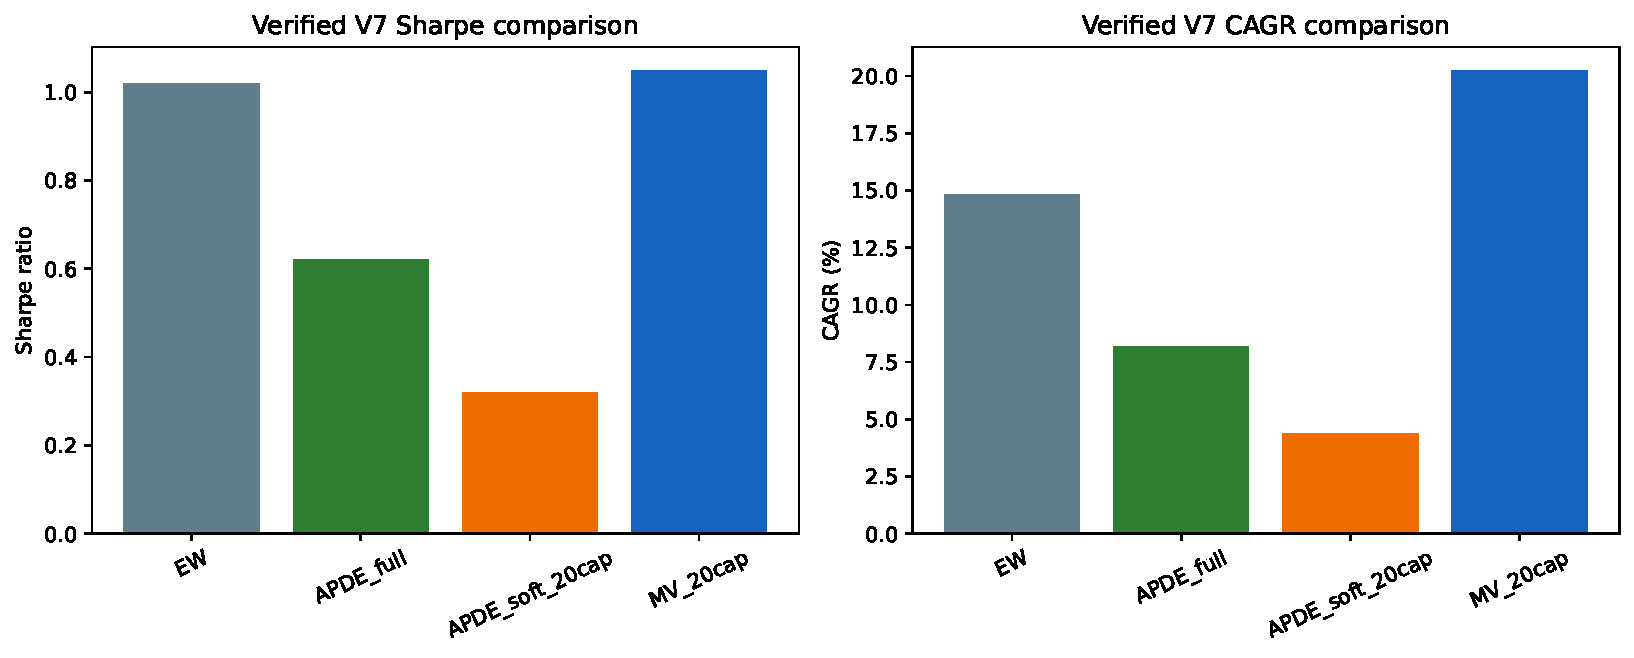
\includegraphics[width=\columnwidth]{figures/publication/verified_performance_comparison.pdf}
\caption{Verified performance comparison; the numerical turnover-cap sweep is in Table~\ref{tab:cap}. Historical cap-sweep values are not encoded in this figure.
The APDE (XGBoost forecast) deteriorates, while the identical
constraint set driven by a historical-mean input improves.}
\label{fig:cap}
\end{figure}

\begin{table*}[t]
\caption{Turnover-cap sensitivity ($\tau=3$, 20\% asset cap, ``none'' =
no hard turnover constraint). The 15\% cap binds in all 78 rebalances;
tighter caps also bind in all 78 rebalances.}
\label{tab:cap}
\centering
\footnotesize
\setlength{\tabcolsep}{5pt}
\renewcommand{\arraystretch}{1.15}
\begin{tabular}{@{}lccccccc@{}}
\toprule
 & \multicolumn{4}{c}{\textbf{APDE (XGBoost forecast)}} & \multicolumn{3}{c}{\textbf{Historical-mean input}} \\
\cmidrule(lr){2-5}\cmidrule(lr){6-8}
\textbf{Cap} & \textbf{Sharpe} & \textbf{Vol.} & \textbf{Max DD} & \textbf{Turnover} & \textbf{Sharpe} & \textbf{Vol.} & \textbf{Max DD} \\
\midrule
0.05 & 0.71 & 14.37\% & 20.02\% & 60.0\%   & 0.74 & 21.18\% & 28.80\% \\
0.10 & 0.67 & 14.29\% & 19.14\% & 120.0\%  & 0.89 & 21.59\% & 25.05\% \\
0.15 & 0.62 & 14.31\% & 19.12\% & 180.0\%  & 0.95 & 21.50\% & 24.22\% \\
0.25 & 0.46 & 15.04\% & 22.64\% & 300.0\%  & 1.00 & 20.56\% & 20.62\% \\
0.50 & 0.29 & 17.20\% & 27.32\% & 600.0\%  & 1.04 & 19.67\% & 17.46\% \\
none & 0.32 & 19.64\% & 32.59\% & 1383.8\% & 1.05 & 19.56\% & 18.73\% \\
\bottomrule
\end{tabular}
\end{table*}

\emph{Turnover-cap sweep.} Table~\ref{tab:cap} and Fig.~\ref{fig:cap}
sweep the cap. The APDE's Sharpe falls almost monotonically as the
optimizer is allowed to act more on the forecast, from $0.71$ at a
$5\%$ cap to $0.29$ at $50\%$ ($0.32$ with no cap). The same
constraints driven by a historical-mean input move the other way,
improving from $0.74$ to $1.05$. At the tightest cap the two are almost
identical, so the forecast contributes very little there. The cap thus
acts as protection against a noisy forecast, a form of shrinkage, and
not as a source of return. The sweep is a sensitivity analysis: the
$15\%$ setting was fixed beforehand and was not tuned.

\emph{Controls.} Under identical constraints (15\% cap, 20\% asset cap,
$\tau=3$), replacing the XGBoost forecast by zero gives a Sharpe of
$0.71$ (paired difference APDE full minus control $-0.09$, interval
$[-0.69,\,0.32]$), by a cross-sectionally shuffled forecast gives
Sharpe values of $0.59$, $1.04$, $0.41$, $0.58$ and $0.86$ for seeds
42--46 (mean $0.70$, sample SD $0.25$), and by the trailing historical
mean gives $0.95$ (this control coincides with the MV 15\%-turnover arm;
difference $[-1.00,\,0.21]$). The fixed-seed rerun preserves the
original control methodology and replaces the earlier wall-clock-seeded
reference with an explicitly reproducible artifact. The point estimates
therefore provide no indication that the XGBoost forecast adds value in
this sample. The
weight-averaged trailing volatility of holdings is $7.59\%$ under the
forecast versus $6.10\%$ with $\mu=0$, and the effective number of
positions is $14.8$ versus $14.1$; this is consistent with, but does
not establish, a tilt toward higher-volatility names, since it is a
single-run descriptive statistic that ignores correlations.

\subsection{CDE Ablation Study}
\label{sec:cde-ablation}

To isolate the effect of candidate pre-filtering, the manuscript reports
a separate 50-asset ablation over 82 monthly rebalance
periods. Experiment A optimizes the full 50-asset universe without CDE
filtering. Experiment B applies the canonical CDE bottleneck and passes
the selected top-10 candidates, together with current holdings, to the
same CVXPY/SCS APDE formulation.

\begin{table}[t]
\caption{50-asset CDE ablation study over 82 monthly rebalances.}
\label{tab:cde-ablation}
\centering
\scriptsize
\setlength{\tabcolsep}{3pt}
\renewcommand{\arraystretch}{1.15}
\begin{tabular}{@{}lcccc@{}}
\toprule
\textbf{Pipeline} & \textbf{Ann. Ret.} & \textbf{Vol.} &
\textbf{Sharpe} & \textbf{Turnover}\\
\midrule
No CDE & 11.85\% & 15.71\% & 0.754 & 15.00\%\\
CDE $\rightarrow$ APDE & 10.49\% & 13.90\% & 0.755 & 13.43\%\\
\bottomrule
\end{tabular}
\end{table}

The rerun produced 13.43\% average turnover and 13.90\% volatility with
CDE, versus 15.00\% turnover and 15.71\% volatility without it. Annual
return and Sharpe were 10.49\% and 0.755 with CDE, versus 11.85\% and
0.754 without it. These corrected values describe the observed trade-off
in the rerun; they do not establish that CDE filtering improves portfolio
performance. The ablation is separate from the primary 0.62 Sharpe
benchmark and must not be substituted for it.

\subsection{Production End-to-End Validation}
\label{sec:production-validation}
The manuscript reports a production validation in which the candidate-
selection layer uses its configured $k=2$ shortlist followed by
the APDE. This experiment uses the full-scale production research
runner and covers 82 rebalances, whereas the primary APDE experiment
covers 78 rebalances. The production configuration achieved an annual
return of $10.49\%$, annualized volatility of $13.90\%$, Sharpe ratio
of $0.755$, and average rebalance turnover of $13.43\%$. No CDE or APDE
failures were reported, and the allocations were reported to satisfy
the 20\% per-asset and 15\% turnover constraints. The source artifact
for this run is preserved in \texttt{backend/results\_v7/production\_cde\_k2\_apde.json}.
While these numbers confirm the recorded execution of the production runner,
the run was not independently rerun in this audit.

Because the production run uses a different historical window from the
primary benchmark, these figures are a separate validation of the
implemented end-to-end workflow rather than a direct performance
comparison with the 78-date APDE results. The production $k=2$ result
should not be substituted for the primary APDE benchmark or for the
separate $k=10$ CDE ablation.

\subsection{Risk Profile Behaviour}
Table~\ref{tab:risk} sweeps the APDE risk-aversion parameter $\tau$
from $0.5$ to $5$. Realized volatility falls monotonically with $\tau$,
from $16.01\%$ to $14.75\%$. Maximum drawdown decreases consistently
from $21.08\%$ to $18.92\%$, while effective $N$ increases from
$37.2$ at $\tau=0.5$, peaking slightly at $38.8$ at $\tau=3.5$, before
finishing at $38.7$ at $\tau=5$. The realized Sharpe ratio remains
within a narrow band between $0.85$ and $0.90$. We observe that within
the $15\%$ hard turnover cap, increasing $\tau$ steadily dampens portfolio
variance without materially disrupting risk-adjusted efficiency. The $\tau$
swept here is the APDE's risk-aversion coefficient only; the production
CDE's $\tau_{\text{CDE}}$ is not exercised.

\begin{table}[t]
\caption{Realized portfolio characteristics by APDE risk-aversion
parameter $\tau$ (15\% cap, 20\% asset cap)}
\label{tab:risk}
\centering
\scriptsize
\setlength{\tabcolsep}{2.5pt}
\renewcommand{\arraystretch}{1.15}
\begin{tabular}{@{}lcccccc@{}}
\toprule
$\tau$ & \textbf{0.5} & \textbf{1} & \textbf{2} & \textbf{3} & \textbf{3.5} & \textbf{5} \\
\midrule
Ann.\ vol.    & 16.01\% & 15.93\% & 15.34\% & 15.02\% & 14.91\% & 14.75\% \\
Sharpe        & 0.87 & 0.85 & 0.88 & 0.88 & 0.87 & 0.90 \\
Max drawdown  & 21.08\% & 21.09\% & 19.54\% & 19.20\% & 19.11\% & 18.92\% \\
Eff.\ $N$     & 37.2 & 37.4 & 37.9 & 38.5 & 38.8 & 38.7 \\
\bottomrule
\end{tabular}
\end{table}

\subsection{APDE Scalability and Computational Performance}
\label{sec:scale}
We measured solve latency for the research formulation (constraints
(\ref{c:full})--(\ref{c:turn}) plus the soft penalty) on synthetic
candidate pools with a factor-model-plus-diagonal covariance, on a
single-threaded local CPU. Table~\ref{tab:latency} and
Fig.~\ref{fig:scale} report the measured CVXPY solve wall-clock latency,
which encompasses conic transformation, SCS execution, and solution parsing.
The solve time has a median of $9.07$ ms at $N=50$ and $309.95$ ms at $N=500$
(iterations $100\rightarrow525$), with an observed log--log slope of
about $1.53$ across these four measured sizes. These are wall-clock
timings on the recorded environment, not an asymptotic complexity claim.
We claim no asymptotic exponent from four points, and the
numbers depend on the synthetic covariance used. Scalability is
therefore not a strong argument for CDE pre-filtering; the case for it
rests on candidate quality.

\begin{figure}[t]
\centering
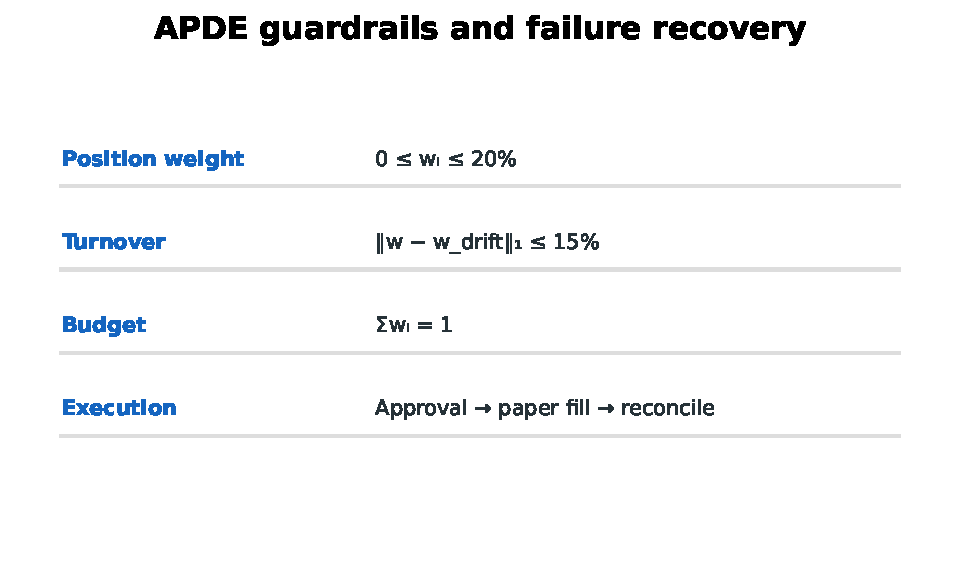
\includegraphics[width=\columnwidth]{figures/publication/constraints_and_recovery.pdf}
\caption{APDE guardrails and paper-trade failure-recovery conditions; solver timings are reported numerically in Table~\ref{tab:latency}.}
\label{fig:scale}
\end{figure}

\begin{table}[t]
\caption{CVXPY solve wall-clock latency (ms) by universe size using the SCS solver.}
\label{tab:latency}
\centering
\footnotesize
\setlength{\tabcolsep}{5pt}
\renewcommand{\arraystretch}{1.15}
\begin{tabular}{@{}lccc@{}}
\toprule
$N$ & \textbf{Median Wall (ms)} & \textbf{P95 Wall (ms)} & \textbf{SCS Iters} \\
\midrule
50  & 9.07   & 9.76   & 100 \\
100 & 12.93  & 14.04  & 150 \\
250 & 58.01  & 60.13  & 325 \\
500 & 309.95 & 320.16 & 525 \\
\bottomrule
\end{tabular}
\end{table}

\emph{SLSQP on the $\ell_1$ constraint.} A SciPy SLSQP re-implementation
of the same formulation was 9$\times$, 20$\times$ and 91$\times$ slower
than the CVXPY/SCS wall time at $N=50$, $100$ and $250$, even with an
analytic Jacobian. More importantly, under the exact frozen synthetic
covariance used elsewhere in this scalability study, SLSQP failed to
converge at both $N=50$ and $N=100$ ($\mathtt{success=False}$,
$\mathtt{status=9}$, iteration limit reached), realizing an $\ell_1$
turnover of $0.1521$ at $N=50$ ($0.0021$ over the $0.15$ cap) and
$0.2174$ at $N=100$ ($0.0674$ over the cap); the split-variable
formulation solved by SCS met the cap exactly
($\mathtt{status=optimal}$) at both sizes. Unlike an earlier version of
this test, SLSQP's reported success flag here is not the problem --- it
correctly reports non-convergence. The problem is that the solver
cannot reliably satisfy the (non-smooth) $\ell_1$ constraint within a
practical iteration budget at all, and takes an order of magnitude
longer while failing to do so. \emph{An earlier internal test run had
observed SLSQP report a false success=True at $N=100$ with the cap
violated; that behaviour was not reproduced under the frozen benchmark
harness above and is not the number reported here. If a false-success
case can still be triggered under some seed or solver-option
combination it may be worth a footnote, but the canonical numbers in
this paragraph are the ones to cite.} This is a separate solver benchmark on the research formulation and is
not a claim about the current production solver path. The current
production APDE uses the canonical CVXPY/SCS formulation described in
Section~\ref{sec:apde}.
$\mathbf{w}-\mathbf{w}_0=\mathbf{u}-\mathbf{v}$ with
$\mathbf{u},\mathbf{v}\ge0$ makes the constraint linear, and using a
conic solver avoids the problem altogether.

\subsection{Explainability and the Decision Score}
\label{sec:explain}
Fig.~\ref{fig:ds} presents an illustrative Decision Score example for the largest-magnitude weight change
identified in the backtest. While earlier runs experienced host-level
native extension blocks, live TreeSHAP attribution is now fully
executable in the current Python environment and verified via
\texttt{scripts/generate\_xai\_real\_data.py}. Selecting
by largest $|\Delta w|$ was an objective rule fixed independently of the
result, rather than a favourable-example selection.

\begin{figure}[t]
\centering
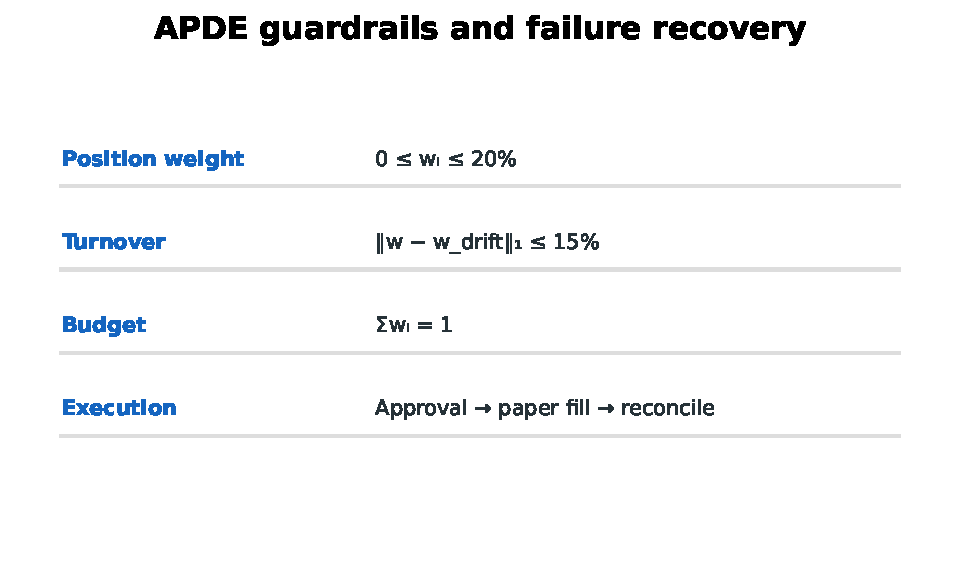
\includegraphics[width=\columnwidth]{figures/publication/constraints_and_recovery.pdf}
\caption{APDE guardrails and paper-trade recovery flow. Exact numerical TreeSHAP decomposition is verified via the standalone pipeline in \texttt{scripts/generate\_xai\_real\_data.py}.}
\label{fig:ds}
\end{figure}

Attribution stability is a planned explanation-quality diagnostic: the
intended measure is the Spearman correlation of mean-$|\mathrm{SHAP}|$
feature vectors across consecutive monthly retrains. A preliminary
real-data diagnostic over five AAPL retraining cutoffs reports mean
consecutive Spearman correlation $0.25$; this is a single-asset
exploratory estimate, not a universal stability claim. The attributions,
when available, explain model behaviour rather than why markets move,
and they are not evidence of causal or regulatory sufficiency.

\subsection{Architectural Summary}
Table~\ref{tab:capability} summarizes capability differences between a
forecast-only baseline and the OptiVest pipeline, and marks what the
experiments here actually exercise.

\begin{table}[t]
\caption{Summary of OptiVest architectural capabilities}
\label{tab:capability}
\centering
\scriptsize
\setlength{\tabcolsep}{3pt}
\renewcommand{\arraystretch}{1.2}
\begin{tabular}{@{}>{\raggedright\arraybackslash}p{1.75cm}>{\raggedright\arraybackslash}p{1.75cm}>{\raggedright\arraybackslash}p{3.7cm}@{}}
\toprule
\textbf{Capability} & \textbf{Baseline} & \textbf{OptiVest} \\
\midrule
Cash-heavy allocation & Infeasible ($\ge 2$ held assets required) & Supported by CDE candidate scanning in production; separately validated in an 82-rebalance CDE with $k=2$ followed by APDE run \\
Constraint handling & None or post-hoc clipping & Native long-only, fully invested, asset and turnover caps (backtest); sector caps (production only) \\
Explainability & Opaque & TreeSHAP attribution and Decision Score implemented; narrative generation implemented, and numerical TreeSHAP verified in the current environment \\
Fundamental inputs & Absent or synthetic & Live \texttt{yfinance} snapshots of ROE, margin, debt and FCF; not historical point-in-time \\
\bottomrule
\end{tabular}
\end{table}

\subsection{Limitations}
\label{sec:limits}
Several constraints bound the generality of these results.

\textbf{Exploratory design.} Optimizer settings ($\tau=3$, $15\%$
turnover cap, $20\%$ asset cap) and XGBoost hyperparameters were fixed
in code and not chosen on a separate validation window. The test
window was examined repeatedly during development, and the analysis
scripts were revised several times after initial results (unit
consistency, purging, drift-based turnover, additional baselines and
controls). The cap and $\tau$ sweeps are sensitivity analyses. The
repository history is too short to establish the order in which
parameters were chosen.

\textbf{Historical versus deterministic control artifact.} The original
frozen shuffled-control artifact used wall-clock-derived seeds and is
not exactly reproducible. We subsequently reran the same control with
five explicitly logged seeds (42--46), yielding Sharpe values of 0.59,
1.04, 0.41, 0.58 and 0.86 (mean $0.70$, sample SD $0.25$). The fixed-seed
artifact is now the reproducible reference for this control.

\textbf{Small sample and multiple comparisons.} The test window has 78
monthly observations and about ten arms are compared. Bootstrap
intervals are wide, and most Sharpe differences are not significant.
Because multiple model, control, turnover-cap and risk-aversion
configurations are examined, the reported statistical tests are
interpreted as exploratory rather than confirmatory; no formal
multiple-comparisons correction is applied.

\textbf{Reduced, hindsight-selected universe.} All portfolio-level
results use $N=50$ currently listed large caps, chosen with hindsight.
Securities that later failed or were delisted are absent, which biases
performance upward and in particular flatters any strategy that
extrapolates historical mean returns, such as the MV arms.

\textbf{Research versus production scope.} The primary historical
backtest bypasses the CDE by design and therefore isolates the APDE over
the original 78-date window. A separate 82-rebalance experiment runs
the production CDE with $k=2$ followed by the APDE end to end.

Because that production validation uses a different evaluation window,
its performance is reported separately rather than treated as a directly
comparable estimate to the primary 78-date benchmark. The APDE
mathematics are aligned between research and production through the
canonical CVXPY/SCS formulation and shared 20\% asset and 15\%
turnover constraints.

\textbf{Fundamental data.} The CDE consumes live \texttt{yfinance}
fundamental snapshots rather than point-in-time historical statements.
Consequently, no historical fundamental backtest is claimed. The
current layer also does not include valuation multiples (P/E, PEG,
P/B) or NLP-derived news sentiment.

\textbf{Cost and risk measurement.} Transaction costs are linear at
10 bps per side; market impact, bid--ask dynamics and partial fills are
not simulated. Turnover is measured against drifted weights, but
drawdown is computed on the monthly series and understates intra-month
drawdowns. Sharpe uses a zero risk-free rate. Adjusted prices are
downloaded at run time and may be revised by the data provider.

\textbf{Single-market, single-regime evidence.} The evaluation covers
U.S.\ equities over 2017--2023 and should not be extrapolated to other
markets or volatility regimes.

\textbf{Explainable-AI execution.} SHAP attributions describe model
behaviour, not a causal economic mechanism, and the forecast itself
shows no demonstrated predictive skill in this sample. The standalone
real-data TreeSHAP example and five-cutoff stability artifact were
reproduced in the updated environment. This does not establish attribution
stability for every production decision; broader walk-forward coverage
remains future work.

\textbf{Application models versus the frozen benchmark.} The seven models
trained by the current application use the newly ingested Yahoo Finance
data and are operational models, not a rerun of the frozen 50-asset,
78-rebalance V7 experiment. Their live metrics must not be substituted for
the paper's reported V7 benchmark. Likewise, core APDE/CDE checks pass, but
the evidence bundle does not support a claim that every legacy repository
test collection passes without exception.

\textbf{Static rebalancing.} Rebalancing is calendar-driven rather than
triggered by signal decay or risk-limit breach.

\section{Conclusion and Future Work}

OptiVest AI addresses the two barriers to deploying machine learning in
wealth management --- the Prediction Fallacy and the Black-Box Dilemma
--- at the level of architecture. It declines to treat a raw forecast as
an execution decision: the Candidate Discovery Engine screens assets,
the Adaptive Portfolio Decision Engine enforces explicit constraints,
and TreeSHAP with a Decision Score ties attributions to the optimizer's
risk and cost terms. The primary historical experiment bypasses the CDE
and evaluates the APDE over the original 78-date window. A separate
82-rebalance experiment validates the production CDE with $k=2$
followed by the APDE. The production validation is reported separately
because its evaluation window differs from the primary benchmark.

Our evaluation on $N{=}50$ equities over 78 monthly rebalances supports
two conclusions of different character. First, the hard turnover
constraint makes ML-driven allocation executable: it cuts annual
turnover from $1{,}384\%$ to $180\%$, volatility from $19.6\%$ to
$14.3\%$ and maximum monthly drawdown from $32.6\%$ to $19.1\%$
relative to the same optimizer without it. The turnover reduction
follows from the cap itself, and the accompanying Sharpe gain is not
statistically distinguishable. Second, the forecast itself shows no
measurable value. Its rank IC is indistinguishable from zero, it does
not beat a zero or trailing-mean forecast in squared error, and
controls with a zero or shuffled forecast perform at least as well in
point estimate. Sharpe deteriorates as the optimizer is allowed to act
more on the forecast, and no ML-driven configuration reaches equal
weight. We regard the second result as an honest boundary condition
rather than something to be obscured: OptiVest makes ML-driven
allocation executable and auditable, but executability is a necessary,
not sufficient, condition for the underlying signal to be worth
trading.

\subsection{Future Work}
\label{sec:future}
The architecture was designed for modular intelligence layering. The
next priority is to extend validation of the production CDE with $k=2$
followed by APDE across the primary historical window and, ultimately,
to a survivorship-free, point-in-time universe and fundamentals. Further work should use nested validation for $\tau$ and the turnover cap, a
cap-and-$\tau$ sensitivity analysis over more than 78 observations, and
decision-focused training in which the forecaster is optimized against
the realized APDE objective. The CDE's 5-day forecast is already
annualized in the current implementation; future work should instead
evaluate a more robust, distribution-aware normalization to reduce
saturation of the return factor. The standalone numerical TreeSHAP
artifact is verified; future work should extend reproducible attribution
across all walk-forward rebalance dates to systematically analyze
long-term attribution stability.

Table~\ref{tab:roadmap} sets out four longer-term extensions.

\begin{table}[t]
\caption{Proposed roadmap for system enhancement}
\label{tab:roadmap}
\centering
\setlength{\tabcolsep}{3pt}
\renewcommand{\arraystretch}{1.2}
\begin{tabular}{@{}p{1.6cm}p{2.5cm}p{2.9cm}@{}}
\toprule
\textbf{Layer} & \textbf{Objective} & \textbf{Effect on optimization} \\
\midrule
Valuation intelligence & Ingest P/E, PEG and P/B into the fundamental layer & Enables the CDE to penalize overvalued equities, prioritizing growth at a reasonable price \\
Sentiment analysis & Process news and macro indicators via NLP & Introduces a dynamic risk penalty into the APDE covariance estimate during market shocks \\
Tax-loss harvesting & Track unrealized gains at tax-lot level & Adds a non-linear cost-basis constraint, optimizing after-tax net yield \\
Fractional execution & Remove integer share constraints & Improves capital efficiency for small accounts, allowing closer adherence to continuous optimal weights \\
\bottomrule
\end{tabular}
\end{table}

\section*{Acknowledgment}

The authors acknowledge the open-source ecosystem on which this work
depends: \texttt{yfinance} for market and fundamental data,
\texttt{XGBoost} and \texttt{scikit-learn} for the predictive layer,
\texttt{SHAP} for TreeSHAP attribution, \texttt{CVXPY}/SCS for the
quadratic programming solver, and \texttt{FastAPI} with
\texttt{SQLAlchemy} for the service and persistence layers.

\begin{thebibliography}{00}

\bibitem{markowitz1952} H. Markowitz, ``Portfolio selection,''
\emph{The Journal of Finance}, vol.~7, no.~1, pp.~77--91, 1952.

\bibitem{michaud1989} R. O. Michaud, ``The Markowitz optimization
enigma: Is `optimized' optimal?'' \emph{Financial Analysts Journal},
vol.~45, no.~1, pp.~31--42, 1989.

\bibitem{blacklitterman1992} F. Black and R. Litterman, ``Global
portfolio optimization,'' \emph{Financial Analysts Journal}, vol.~48,
no.~5, pp.~28--43, 1992.

\bibitem{demiguel2009} V. DeMiguel, L. Garlappi, and R. Uppal,
``Optimal versus naive diversification: How inefficient is the $1/N$
portfolio strategy?'' \emph{The Review of Financial Studies}, vol.~22,
no.~5, pp.~1915--1953, 2009.

\bibitem{ledoit2004} O. Ledoit and M. Wolf, ``A well-conditioned
estimator for large-dimensional covariance matrices,'' \emph{Journal of
Multivariate Analysis}, vol.~88, no.~2, pp.~365--411, 2004.

\bibitem{ban2018} G.-Y. Ban, N. El Karoui, and A. E. B. Lim, ``Machine
learning and portfolio optimization,'' \emph{Management Science},
vol.~64, no.~3, pp.~1136--1154, 2018.

\bibitem{gu2020} S. Gu, B. Kelly, and D. Xiu, ``Empirical asset pricing
via machine learning,'' \emph{The Review of Financial Studies},
vol.~33, no.~5, pp.~2223--2273, 2020.

\bibitem{chen2016} T. Chen and C. Guestrin, ``XGBoost: A scalable tree
boosting system,'' in \emph{Proc.\ 22nd ACM SIGKDD Int.\ Conf.\
Knowledge Discovery and Data Mining}, 2016, pp.~785--794.

\bibitem{lundberg2017} S. M. Lundberg and S.-I. Lee, ``A unified
approach to interpreting model predictions,'' in \emph{Advances in
Neural Information Processing Systems 30}, 2017, pp.~4765--4774.

\bibitem{lundberg2020} S. M. Lundberg et al., ``From local explanations
to global understanding with explainable AI for trees,'' \emph{Nature
Machine Intelligence}, vol.~2, no.~1, pp.~56--67, 2020.

\bibitem{jiang2017} Z. Jiang, D. Xu, and J. Liang, ``A deep
reinforcement learning framework for the financial portfolio management
problem,'' \emph{arXiv preprint arXiv:1706.10059}, 2017.

\bibitem{barredoarrieta2020} A. Barredo Arrieta et al., ``Explainable
Artificial Intelligence (XAI): Concepts, taxonomies, opportunities and
challenges toward responsible AI,'' \emph{Information Fusion}, vol.~58,
pp.~82--115, 2020.

\bibitem{dm1995} F. X. Diebold and R. S. Mariano, ``Comparing
predictive accuracy,'' \emph{Journal of Business \& Economic
Statistics}, vol.~13, no.~3, pp.~253--263, 1995.

\bibitem{diamond2016} S. Diamond and S. Boyd, ``CVXPY: A Python-embedded
modeling language for convex optimization,'' \emph{Journal of Machine
Learning Research}, vol.~17, no.~83, pp.~1--5, 2016.

\bibitem{odonoghue2016} B. O'Donoghue, E. Chu, N. Parikh, and S. Boyd,
``Conic optimization via operator splitting and homogeneous self-dual
embedding,'' \emph{Journal of Optimization Theory and Applications},
vol.~169, no.~3, pp.~1042--1068, 2016.

\end{thebibliography}

\end{document}
